
%============================= HEADER =================================
\chapter{Radiative Transfer}\label{ch:iii}

\section{Introduction}

Most of our knowledge about the Universe is based on the electromagnetic radiation that reaches us from far far away. EM radiation is obviously not the only way we can probe the Universe we live in but, in respect to neutrinos, cosmic rays or even gravitational waves, it's not a long stretch to claim it is by far the most understood.
\par It is most important then that an astrophysicist worthy of his (or her) name has a good grasp of the theory of radiative transfer and of its applications.
\par Apart from a few more key differences, I'll follow the description of radiative transfer of \cite{choudhuri} and \cite{1986rpa..book.....R}, but I won't fail to emphasize whenever I'll be doing otherwise.

\section{Relevant quantities for radiative transfer}

Although some books often start their description of radiative transfer from the definition of \emph{monochromatic energy} and \emph{monochromatic intensity}, I found that it is most misleading, since, in all but a few cases, what we experimentally measure are fundamentally \emph{fluxes}. 
\par We shall then consider the \emph{monochromatic flux} $F_{\nu}$ ($\text{erg}\,\text{s}^{-1}\,\text{Hz}^{-1}\,\text{cm}^{-2}$) produced by some source passing through a small area $\text{d}A$ located somewhere in space. 
\begin{figure}[h!]
	\centering
	\includegraphics[width=0.7\textwidth]{img/radcostruction.png}
	\caption{Schematic geometrical representation of the system. \\Credits: \cite{1986rpa..book.....R}.}
\end{figure}
\par If we call \textbf{$\hat{k}$} the propagation direction of the flux and \textbf{$\hat{n}$} the unit vector emerging from the surface $\text{d}A$, it's easy to get convinced that what is actually passing through the surface is something proportional to $F_{\nu} (\textbf{$\hat{k}$} \cdot \textbf{$\hat{n}$})$.
\par From the monochromatic flux we can define the \emph{bolometric flux}, which is just the monochromatic flux integrated over all frequencies (or wavelengths)
\begin{equation}
	F = \int_{0}^{+\infty} F_{\nu}\, \text{d}\nu = \int_{0}^{+\infty} F_{\lambda}\, \text{d}\lambda
\end{equation}
This also tells us how to convert a flux per unit frequency to a flux per unit wavelength
\begin{equation*}
	 F_{\nu}\, \text{d}\nu = F_{\lambda}\, \text{d}\lambda
\end{equation*}
\par By now it should be clear that, despite being experimentally sensible to use the flux, we're losing much information sticking with it, namely directional information.
\par We consider then the amount of radiation $E_{\nu}\,\text{d}\nu$ passing through the same area in time $\text{d}t$ and solid angle $\text{d}\Omega$. Hence we can write
\begin{equation}
	\text{d}E_{\nu}\,\text{d}\nu = I_{\nu}(\textbf{r}, t, \textbf{$\hat{k}$}) (\textbf{$\hat{k}$} \cdot \textbf{$\hat{n}$}) \, \text{d}t \, \text{d}\Omega \, \text{d}A \, \text{d}\nu
    \label{eq:specificmonochromaticintensity}
\end{equation}
where the quantity $I_{\nu}(\textbf{r}, t, \textbf{$\hat{k}$})$ is called the \emph{specific monochromatic intensity}. If $I_{\nu}(\textbf{r}, t, \textbf{$\hat{k}$})$ is specified for all directions at every point in a certain region of spacetime, then we'd have a complete prescription of the radiation field we intend on studying.
\par Capitalizing on the blatant similarities with distribution functions, we can evaluate the moments of the monochromatic intensity.
\begin{definition}{Monochromatic mean intensity $J_{\nu}$}
	\begin{equation*}
		J_{\nu} = \frac{1}{4\pi} \int_{\Omega} I_{\nu}\, \text{d}\Omega = \frac{c}{4\pi} U_{\nu}
	\end{equation*}
	with $U_{\nu}$ the total energy density of radiation.
	Note that $J_{\nu}$ is essentially just an average of the monochromatic intensity over all solid angles.
\end{definition}
\begin{definition}{Monochromatic flux $\vec{F}_{\nu}$}
	\begin{equation*}
		\vec{H}_{\nu} = \frac{1}{4\pi} \int_{\Omega} I_{\nu}(\textbf{$\hat{k}$})\textbf{$\hat{k}$}\, \text{d}\Omega \implies  \frac{1}{4\pi} F_{\nu} = \vec{H}_{\nu}\cdot \hat{n}
	\end{equation*}
	I haven't explicitly proved the last equality, but it shouldn't be hard for you to convince yourself (or prove it yourself) that it is indeed true.
\end{definition}
\begin{definition}{Monochromatic radiation pressure $p_{\nu}$}
	The monochromatic pressure is defined starting from the different directions correlations of the monochromatic intensity 
	\begin{equation*}
		K_{\nu}^{ij} = \frac{1}{4\pi} \int_{\Omega} I_{\nu}(\textbf{$\hat{k}$})\textbf{$n^{i}$}\textbf{$n^{j}$}\, \text{d}\Omega 
	\end{equation*}
	The pressure in particular is usually expressed as
	\begin{equation*}
		P_{\nu} = \frac{1}{c} \int_{\Omega} I_{\nu}(\textbf{$\hat{k}$}) \cos^{2}\theta\,\text{d}\Omega
	\end{equation*}
	where $\cos^{2}\theta = (\textbf{$\hat{k}$} \cdot \textbf{$\hat{n}$})^{2}$.
\end{definition}
In particular, note that for an isotropic field $I_{\nu}$, the average brightness $J_{\nu}$ is one and the same with the monochromatic specific intensity
\begin{equation*}
    J_{\nu} = I_{\nu} \quad (\text{if the field is isotropic})
\end{equation*}

\section{Blackbody Function}

Even at an undergraduate level, we're all fairly familiar with \emph{blackbody radiation}. The easiest way to deduce the expression for the energy density of photons in \emph{thermal equilibrium} (STE) inside a cavity is by the means of statistical mechanics.
\par Remember the Bose-Einstein distribution ($\mu = 0$)
\begin{equation*}
	n = \frac{1}{\exp(h\nu/kT)-1}
\end{equation*}
and the phase space density of states (per unit volume)
\begin{equation*}
	\rho(\nu)\,\text{d}\nu = \frac{4\pi h g \nu^{3}}{c^{3}}\,\text{d}\nu
\end{equation*}
from which deducing the expression from internal energy is straightforward. Remembering $g=2$ is the quantum degeneracy of photons, a simple moltiplication of the previous expressions yields
\begin{equation}
	U_{\nu}\,\text{d}\nu = \frac{8\pi h}{c^{3}}\frac{\nu^{3}}{\exp(h\nu/kT)-1}\,\text{d}\nu
    \label{eq:blackbody_endens}
\end{equation}
\par The energy of a photon is $E_{\gamma} = h\nu$, meaning the number of photons in the frequency range $\nu \to \nu + \text{d}\nu$ is
\begin{equation}
    n_{\nu}\,\text{d}\nu = \frac{8\pi}{c^{3}}\frac{\nu^{2}}{\exp(h\nu/kT)-1}\,\text{d}\nu
    \label{eq:blackbody_numdens}
\end{equation}
which can be integrated over all frequencies, thus obtaining the number density of photons in blackbody radiation
\begin{equation}
    n_{\gamma} = \beta T^{3} \quad \beta = \frac{2.4041 k^{3}}{\pi^{2}\hbar^{3}c^{3}}
    \label{eq:blackbody_totnum}
\end{equation}
\par Since blackbody radiation is isotropic (it depends only on the absolute temperature $T$), the definition of mean monochromatic intensity yields
\begin{equation}
	\boxed{
	B_{\nu}(T) = \frac{2h\nu^{3}}{c^{2}}\frac{1}{\exp(h\nu/kT)-1}
	}
	\label{eq:blackbodyintensity}
\end{equation}
\begin{figure}[h!]
	\centering
	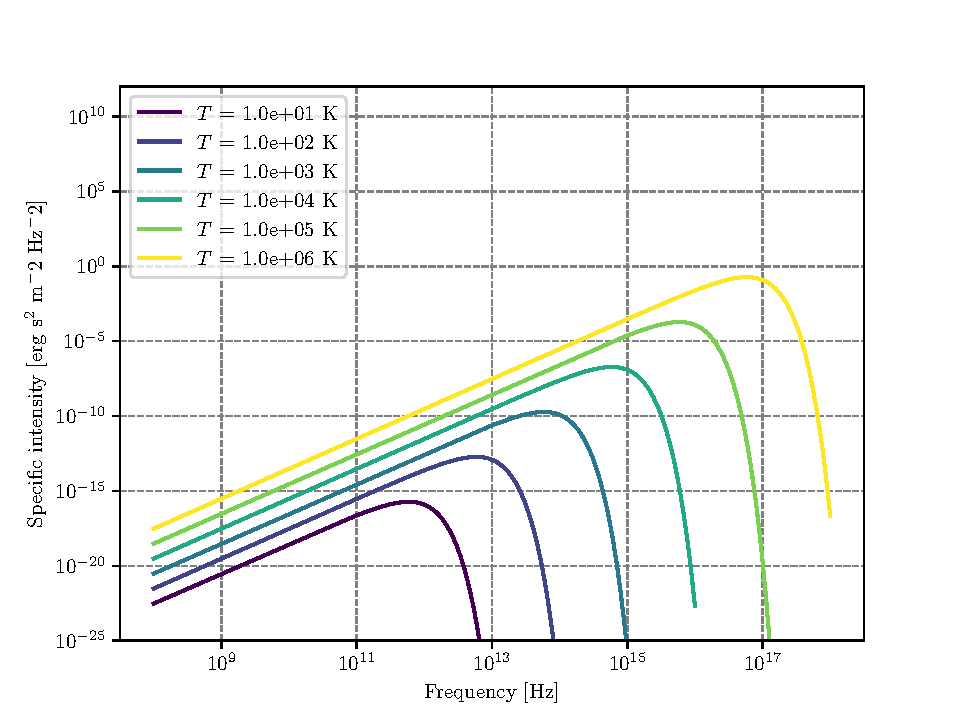
\includegraphics[width=0.9\textwidth]{img/blackbody.pdf}
	\caption{Blackbody frequency spectrum.}
    \label{fgr:planckfunction}
\end{figure}
\par It's important to notice that, in principle, such a fundamental result holds only in \emph{strict thermodynamic equilibrium} (STE), but it's possible to generalize this formulation for less "restrictive" environments.
\par An incredible number of important results descends from (\ref{eq:blackbodyintensity}), and it may be worthwhile to cite at least some of them, starting from Stefan-Boltzmann law. We'll use the following result without proving it 
\begin{equation*}
	\int_{0}^{+\infty} B_{\nu}(T)\,\text{d}\nu = \frac{2h}{c^{2}}\frac{\pi^{4}}{15}\left(\frac{kT}{h}\right)^{4}
\end{equation*}
\par Computing the bolometric flux and the bolometric energy density by integrating over all frequencies using what we've just written down, you find the following 
\begin{equation*}
	U(T) = aT^{4} \quad F(T) = \sigma_{SB}T^{4}
\end{equation*}
\par Clearly the two constants $a$ and $\sigma_{SB}$ cannot be independent, and are actually related by the integral we've previously calculated. Using for example\footnote{The emergent flux from an isotropically emitting surface (such as a blackbody) is $\pi\cdot \text{brightness}$ which is none other than the specific intensity.}
\begin{equation*}
	F(T) = \pi \int_{0}^{+\infty} B_{\nu}(T)\,\text{d}\nu
\end{equation*}
you can easily find out that the \emph{Stefan-Boltzmann constant} is equal to $$ \sigma_{SB} = \frac{2\pi^{5}k^{4}}{15c^{2}h^{3}}$$
and the relation with $a$ is simply $\sigma_{SB} = ac/4$.
\par The equation 
\begin{equation}
	F(T) = \frac{2\pi^{5}k^{4}}{15c^{2}h^{3}} T^{4}
	\label{eq:SB}
\end{equation}
is what is usually known as the \emph{Stefan-Boltzmann law}.
\par Let us now consider two different regimes for eq.\ref{eq:blackbodyintensity}: $h\nu/kT \ll 1$ and $h\nu/kT \gg 1$. The first yields what is commonly known as the Rayleigh-Jeans Law which is, sadly, pretty much relevant only for radioastronomy.
\par Since 
\begin{equation*}
	\exp\left(\frac{h\nu}{kT}\right) = 1+\frac{h\nu}{kT}+o\left(\frac{h\nu}{kT}\right)^{2}
\end{equation*} 
the blackbody radiation assumes the much simpler form of
\begin{equation*}
	B_{\nu}^{RJ} = \frac{2\nu^{2}}{c^{2}}kT
\end{equation*}
\par Another important results is achieved in the opposite regime, when the exponential term is rather larger than unity
\begin{equation*}
	B_{\nu}^{W} = \frac{2h\nu^{3}}{c^{2}}\exp\left(-\frac{h\nu}{kT}\right)
\end{equation*}
This expression is known as Wien's Law.

\subsection*{Characteristic Temperatures}

Starting from the blackbody spectrum we can give various definitions of temperature, that are going to be more and less useful when dealing with stars. The definitions are those of \cite{1986rpa..book.....R}.

\subsubsection*{Brightness Temperature}

One way of characterizing brightness (specific intensity) at a certain frequency is to give the temperature of the blackbody having the same brightness at that frequency. That is, for any value $I_{\nu}$ we define $T_{b}(\nu)$ by the relation
\begin{equation*}
    I_{\nu} = B_{\nu}(T_{b})   
\end{equation*}
this way of specifying brightness has the advantage of being closely connected with the physical properties of the emitter, and has the simple unit (K). This procedure is used especially in radio astronomy, where the Rayleigh-Jeans law is usually applicable.
\begin{equation}
    T_{b} = \frac{c^{2}}{2\nu k}I_{\nu} \quad h\nu/kT \ll 1
    \label{eq:brightnesstemperature-RJ}
\end{equation}
Note that the uniqueness of the definition of brightness temperature relies on the monotonicity property of Planck‘s law. Also note that, in general, the brightness temperature is a function of $\nu$.

\subsubsection*{Color Temperature}

Often a spectrum is measured to have a shape more or less of blackbody form, but not necessarily of the proper absolute value. For example, by measuring $F_{\nu}$, from an unresolved source we cannot find $I_{\nu}$, unless we know the distance to the source and its physical size.
\par By fitting the data to a blackbody curve without regard to vertical scale, a color temperature $T_{c}$, is obtained. Often the “fitting” procedure is nothing more than estimating the peak of the spectrum and applying Wien’s displacement law to find a temperature.

\subsubsection*{Effective Temperature}

The effective temperature of a source $T_{eff}$ is derived from the total amount of flux, integrated over all frequencies, radiated at the source. We obtain $T_{eff}$ by equating the actual flux $F$ to the flux of a blackbody at temperature $T_{eff}$
\begin{equation}
    F = \int I_{\nu}\cos\theta \,\text{d}\nu\,\text{d}\Omega := \sigma T_{eff}^{4}
    \label{eq:effectivetemperature} 
\end{equation}

\section{Radiative transfer equation}

In the presence of matter, it is not immediately obvious what changes may occur in the specific intensity as we move along a ray path. The aim of this section will be to eviscerate the matter.
\par Let's consider the following geometric construction
\begin{figure}[h!]
	\centering
	\includegraphics[width=0.7\textwidth]{img/rtvacuum.png}
	\caption{Geometrical construction for ray paths propagating in empty space. \\ Credits: \cite{1986rpa..book.....R}.}
\end{figure}
\par It won't take a lot of effort to convince yourself that in empty space the monochromatic intensity $I_{\nu}$ is actually conserved. In fact, from simply writing down the definitions and imposing the conservation of energy
\begin{equation*}
	I_{\nu_{2}}\,\text{d}A_{2}\,\text{d}t\,\text{d}\Omega_{2}\,\text{d}\nu = I_{\nu_{1}}\,\text{d}A_{1}\,\text{d}t\,\text{d}\Omega_{1}\,\text{d}\nu
\end{equation*}
the conclusion follows observing that $\text{d}A_{2}\,\text{d}\Omega_{2} = \text{d}A_{1}\,\text{d}\Omega_{1}$.
\par If we consider an affine parameter of the form $\vec{x} = \vec{x}_{0}+\textbf{$\hat{k}$}s$, we may as well write the previous results in a more familiar fashion
\begin{equation}
	\frac{\text{d}I_{\nu}}{\text{d}s} = 0 \implies (\textbf{$\hat{k}$}\cdot \textbf{$\nabla$}) I_{\nu} = 0
	\label{rtvoid}
\end{equation}
\par What changes if matter is present along the ray path? Clearly it will no longer be true that $(\textbf{$\hat{k}$}\cdot \textbf{$\nabla$}) I_{\nu} = 0$, but we're not that far off. All that we need is some little work on both terms.
\par How the right hand side of the equation should change is obvious: It needs to keep track of the "creation" and "destruction" of photons in the considered volume of spacetime.
\par The left hand side of the equation requires a little more care. Consider infinitesimal time and space displacements along the ray path, respectively $\text{d}t$ and $\text{d}\vec{x}$
\begin{equation*}
	\Delta E_{\nu}\,\text{d}\nu = \left(I_{\nu}(\vec{x}+\text{d}\vec{x}, t+\text{d}t, \hat{k})-I_{\nu}(\vec{x}, t, \hat{k})\right)\, \text{d}t \, \text{d}\Omega \, \text{d}A \, \text{d}\nu
\end{equation*}
\par Taking a first order expansion in respect to the affine parameter $s$ along the ray path yields
\begin{equation*}
	\left(\frac{1}{c}\partial_{t}I_{\nu}+\partial_{s}I_{\nu}\right)\, \text{d}t \, \text{d}s\, \text{d}\Omega \, \text{d}A \, \text{d}\nu = \text{photon addition}-\text{photon removal}
\end{equation*}
\par This equation is a generalization of eq.\ref{rtvoid} for non-stationary radiative transport and in the presence of matter. It's about time we get to know what "lives" in the right hand side of the equation.

\subsection{Monochromatic emission coefficient}

For the moment, we'll define the \emph{spontaneous} monochromatic emission coefficient $j_{\nu}$ as
\begin{equation}
	\text{d}E_{\nu}\,\text{d}\nu = j_{\nu}\,\text{d}V\,\text{d}t \, \text{d}\Omega \, \text{d}\nu
	\label{eq:jnu}
\end{equation}
which in general has a non-zero dependence on the emission direction. Sometimes the spontaneous emission coefficient is defined by the \emph{emissivity}\footnote{Please note that often the two names are used almost interchangeably.} $\epsilon_{\nu}$, which is the energy emitted spontaneously per unit frequency per unit time per unit mass
\begin{equation*}
	j_{\nu} = \frac{\epsilon_{\nu}\rho}{4\pi}
\end{equation*}
where $\rho$ is the mass density of the emitting medium.
\par If we perform the decomposition $\text{d}V = \text{d}A\,\text{d}s$, the contribution of spontaneous emission to the specific intensity is
\begin{equation*}
	\text{d}I_{\nu} = j_{\nu}\,\text{d}s
\end{equation*}

\subsection{Absorption coefficient}

Similarly, we can consider the energy that is absorbed from the radiation when passing through a medium. There exists various definitions; I'll use the one we gave in class and that is incidentally the one used in \cite{choudhuri} and \cite{1986rpa..book.....R} as well.
\par We define the \emph{absorption coefficient} $\alpha_{\nu}$ through the following expression
\begin{equation}
	\text{d}I_{\nu} = -\alpha_{\nu}I_{\nu}\,\text{d}s
	\label{eq:alphanu}
\end{equation}
\par If we use a microscopic model, then the absorption coefficient can be understood as particles with numeric density $n$ presenting an effective absorbing area, the \emph{cross section} $\sigma_{\nu}$. The coefficient $\alpha_{\nu}$ can thus be rewritten in terms of
\begin{equation*}
	\alpha_{\nu} = n\sigma_{\nu} = \rho \kappa_{\nu}
\end{equation*}
where $\kappa_{\nu}$ is called the mass absorption coefficient or the \emph{mass-weighed opacity coefficient}.
\par Note that in eq.\ref{eq:alphanu}, we consider “absorption” to include both “true absorption” and stimulated emission, because both are proportional to the intensity of the incoming beam. Depending on the entity of the contribution, the $\alpha_{\nu}$ coefficient may be positive or even negative, giving raise to curious phenomena.
\vspace{0.5cm}
\par Making full use of what we've just defined, we can finally present the celebrated \emph{equation of radiative transfer} (although in the notable absence of scattering)
\begin{equation}
	\frac{\text{d}I_{\nu}}{\text{d}s} = -\alpha_{\nu}I_{\nu}+j_{\nu}
	\label{eq:rt}
\end{equation}
which is actually fairly easy to solve when one of the two coefficients vanishes.

\subsubsection*{Emission only}

We set $\alpha_{\nu} = 0$ and the equation may be solved by direct integration
\begin{equation*}
	I_{\nu}(s) = I_{\nu}(s_{0})+\int_{s_{0}}^{s} j_{\nu}(s')\,\text{d}s'
\end{equation*}
the result is not that interesting per se.

\subsubsection*{Absorption only}

This time we set $j_{\nu} = 0$. The equation is easily solved this time as well 
\begin{equation*}
	I_{\nu}(s) = I_{\nu}(s_{0})\exp\left(-\int_{s_{0}}^{s} \alpha_{\nu}(s')\,\text{d}s'\right)
\end{equation*}
\par In this case, it's rather common to write down the equation in terms of a new variable, the \emph{optical depth}\footnote{Although I don't support this particular choice--since it is bound to create confusion with the mass-weighed opacity $\kappa_{\nu}$--the optical depth is sometimes referred to as simply \emph{opacity}.} $\tau_{\nu}$
\begin{equation}
	\text{d}\tau_{\nu} = -\alpha_{\nu}\,\text{d}s
\end{equation}
which means 
\begin{equation}
    \tau_{\nu} = -\int_{s_{\text{out}}}^{s_{\text{in}}} \alpha_{\nu}(s)\diff{s}
    \label{eq:opticaldepth}
\end{equation}
Given this definition we'll say that if
\begin{itemize}
	\item $\tau_{\nu} \gg 1$: the medium is \emph{optically thick or opaque}
	\item $\tau_{\nu} \ll 1$: the medium is \emph{optically thin or transparent}
\end{itemize}
This has some crucial implications we'll be going through in a moment.
\par In the stationary limit, the equation of radiative transport may be written as 
\begin{equation*}
	(\hat{k}\cdot \nabla)I_{\nu}(\hat{k}, \vec{x}\,) = j_{\nu}(\vec{x}\,)-\alpha_{\nu}(\vec{x}\,)I_{\nu}(\hat{k}, \vec{x}\,)
\end{equation*}
In terms of the \emph{source function} $S_{\nu} = j_{\nu}/\alpha_{\nu}$ it becomes (dropping the functional dependencies for conciseness)
\begin{equation}
	\frac{\text{d}I_{\nu}}{\text{d}\tau_{\nu}} = -I_{\nu}+S_{\nu}
\end{equation}
which can be integrated to yield the formal solution
\begin{equation}
    \boxed{
	    I_{\nu}(\hat{k}, \tau_{\nu}) = I_{\nu}(\tau_{\nu,\,0})\exp(-\tau_{\nu})+\int_{\tau_{\nu,\,0}}^{\tau_{\nu}} d\tau_{\nu}'\,S_{\nu}\exp(-(\tau_{\nu}-\tau_{\nu}'))
    }
    \label{eq:rt-general}
\end{equation}
Assume for the moment that the matter through which radiation is passing has constant properties and has no background source. Then the source function $S_{\nu}$ is constant and the formal equation becomes
\begin{equation*}
	I_{\nu} = S_{\nu}(1-e^{-\tau_{\nu}})
\end{equation*}
If the medium  and is optically thin, then the equation is reduced to 
\begin{equation}
	I_{\nu} = S_{\nu}\tau_{\nu} = j_{\nu}L
\end{equation}
by taking the Taylor expansion of the exponential term and calling $L$ some typical length of the medium.
\par If, on the other hand, the medium is optically thick, we can neglect the exponential $e^{-\tau_{\nu}}$ to obtain
\begin{equation}
	I_{\nu} = S_{\nu}
	\label{eq:k1}
\end{equation}

\section{Kirchhoff's Law and LTE}

The most notable implication of (\ref{eq:k1}) is if we consider the specific intensity coming out of a small hole on a box kept in thermodynamic equilibrium. We know that what's going to come out of there is the blackbody radiation
\begin{equation*}
	I_{\nu} = B_{\nu}(T)
\end{equation*}
but what if we were to put an optically thick object just behind the hole?
\par If the object is in thermodynamic equilibrium with the surroundings (and it \emph{will} be, given an appropriate amount of time), then the radiation coming out of the hole will still be blackbody radiation. But (\ref{eq:k1}) tells us that the source function will tend to be equal to the specific intensity, hence
\begin{equation}
	S_{\nu} = B_{\nu}(T)
\end{equation}
which actually puts a constraint on the possible values of the emission coefficient in terms of the absorption coefficient. This is exactly what is expressed in Kirchhoff's law 
\begin{equation}
    \boxed{
	    j_{\nu} = \alpha_{\nu}B_{\nu}
    }
	\label{eq:kirchhoff}
\end{equation}
Let us briefly consider what we have just derived. Matter often tends to emit and absorb at specific frequencies corresponding to what are commonly called \emph{spectral lines}. We would expect then  both $j_{\nu}$ and $\alpha_{\nu}$ to have peaks (or depressions) around these lines. But Kirchhoff's law forces their ratio to be equal to a smooth blackbody profile.
\par Thus we can expect to observe two very different scenarios if the medium is optically thin rather than optically thick. In the former, the radiation emerging from the medium is essentially determined by its emission coefficient; since $j_{\nu}$ is expected to present peaks, so will the radiation spectrum, which will be appear in spectral lines, as shown in Fig.\ref{fig:emission} and Fig.\ref{fig:absorption}.
\begin{figure}[h!]
	\centering
	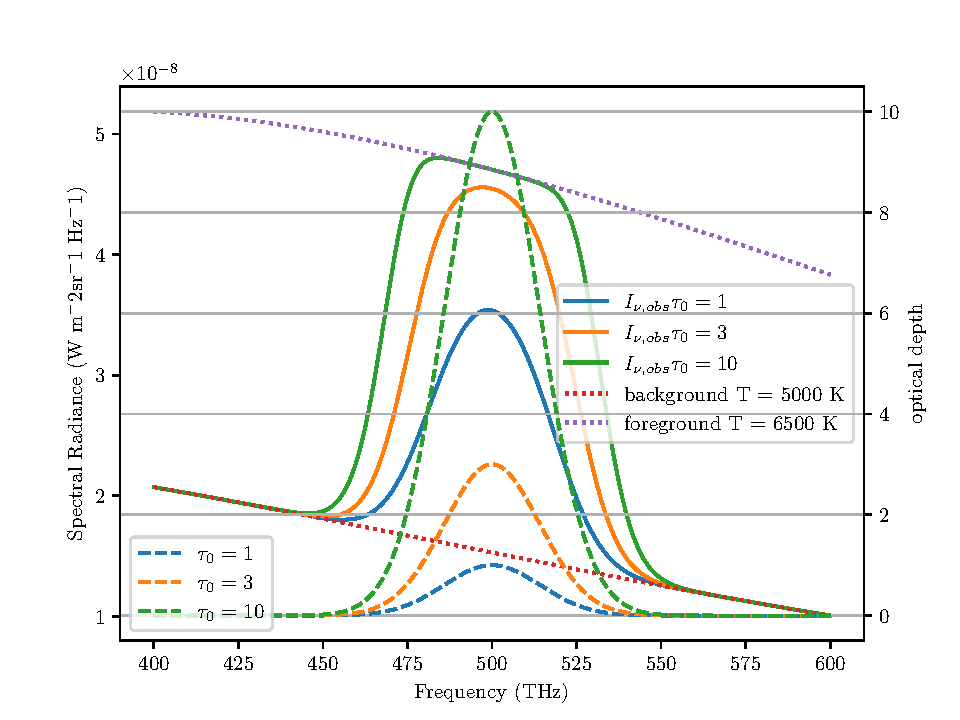
\includegraphics[width=0.8\textwidth]{img/img2.pdf}
	\caption{An example of emission features formation for different temperatures and different values of $\tau$. Credits: Prof. Walter del Pozzo.}
	\label{fig:emission}
\end{figure}
\begin{figure}[h!]
	\centering
	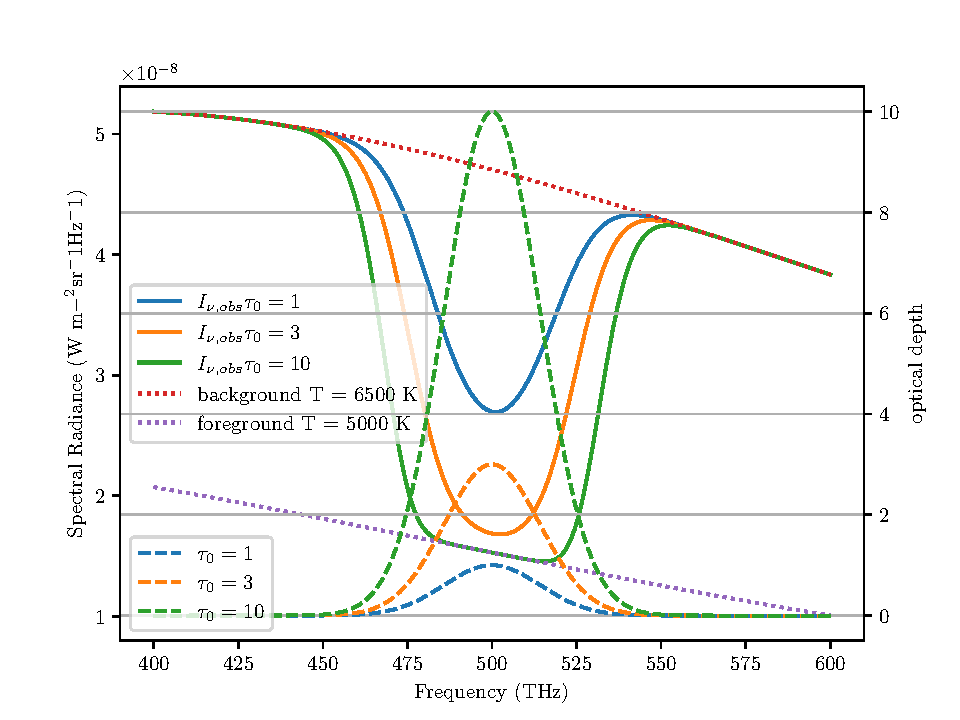
\includegraphics[width=0.8\textwidth]{img/img1.pdf}
	\caption{An example of absorption features formation for different temperatures and different values of $\tau$. Credits: Prof. Walter del Pozzo.}
	\label{fig:absorption}
\end{figure}
\par On the other hand, the intensity coming out of an optically thick body is its source function, which must be equal to the blackbody function. Hence we expect the medium to emit in a continuum, like a blackbody.
\par All throughout this description, we've been assuming the medium to have (global) constant properties, which has the perk of being a good approximation for many objects of interest, but still turns out to be a really poor one for many other objects. Stars, for example. 
\par Ingenuously, we may expect stars to emit radiation like blackbodies, but they're not. Actually, stars present absorption lines, many, even, depending on the class of star. What we cannot assume in stars is them having constant properties, starting from temperature.
\par In fact, we could take a guess and claim that stars are in \emph{strict} thermodynamic equilibrium. It would be a very bad guess indeed.

\subsubsection{Local Thermodynamic Equilibrium (LTE)}

Let's be honest: In a realistic situation, we \emph{rarely} have strict thermodynamic equilibrium. If a body is in thermodynamic equilibrium, we can assume a number of important physical principles to hold, like the Maxwellian distribution 
\begin{equation}
	\text{d}n_{v} = 4\pi n \left(\frac{m}{2\pi k T}\right)^{3/2}v^{2}\exp\left(-\frac{mv^{2}}{2kT}\right)\,\text{d}v
\end{equation}
where $n$ is the total number of particles per unit volume and $m$ is the mass of each particle. Similarly, we can expect certain laws to hold, like Boltzmann's law for occupation numbers
\begin{equation}
	\frac{n_{E}}{n_{0}} = \frac{g_{E}}{g_{0}}\exp\left(-\frac{E-E_{0}}{kT}\right)
    \label{eq:boltmann-occ}
\end{equation}
\par The proverbial "one-million-dollar-question" then is: When can we expect a system to be in thermodynamic equilibrium and when can we expect the previous principles to hold?
\par Even if the system initially does not obey the, say, Maxwellian distribution, it will eventually relax to it after undergoing some \emph{collisions}.
\par \textbf{Collisions are crucial in establishing thermodynamic equilibrium}. 
\par When collisions are frequent, the mean free path of particles will be small, and particles will interact more effectively. When this happens, we can expect the principles aforementioned to hold. Since we're physicists, vague sentences like "\emph{the mean free path of particles will be small}" are destined to elicit a deep sense of unease and distress. How small does the free path have to be? One meter? Two micrometers? Below the Planck lengthscale?
\par When we've defined the absorption coefficient $\alpha_{\nu}$, the sharpest among my four readers total may have noticed that $\alpha_{\nu}$ has the dimension of the inverse of a length. It is safe to assume that $\alpha_{\nu}^{-1}$ may define some distance over which a significant fraction of the radiation would get absorbed by matter.
\par Such a "mean-distance" is defined in a homogeneous medium as 
\begin{equation*}
	\langle \tau_{\nu} \rangle = \alpha_{\nu}l_{\nu} = 1
\end{equation*}
\par Thus, if $l_{\nu}$ is sufficiently small such that the temperature can be taken as a constant over such distance, we can safely say that the useful relations we have defined earlier still hold, although only locally.
\par In such a fortunate scenario, known as \emph{Local Thermodynamic Equilibrium} (LTE), all the important laws requiring thermodynamic equilibrium are expected to hold, provided that we use the local temperature $T(\vec{x}\,)$.
\par In the interiors of stars, for example, LTE will prove to be a very good approximation, that will get progressively worse as we approach the "surface" of the star.
\par Notably, it is possible to show that Kirchhoff's law (\ref{eq:kirchhoff}) is valid also in the LTE regime.
\par Then, if we assume LTE, we can use $S_{\nu} = B_{\nu}(T)$, so that $S_{\nu}$ can be taken out of the integral (\ref{eq:rt-general}) since the blackbody field is isotropic
\begin{equation}
    I_{\nu}(\hat{k}, \tau_{\nu}) = I_{\nu}(\tau_{\nu,\,0})\exp(-\tau_{\nu})+B_{\nu}(T)\left(1-\exp(-\tau_{\nu})\right)
\end{equation}
which is useful to solve in the RJ regime $h\nu/kT \ll 1$ where
\begin{align*}
    B_{\nu}(T) &\approx \frac{2k\nu^{2}}{c^{2}}T\\
    I_{\nu}(\tau_{\nu}) &\textoversymbol{=}{def} B_{\nu}(T_{B}) \approx \frac{2k\nu^{2}}{c^{2}}T_{B}\\
    I_{\nu}(\tau_{\nu,0}) &= B_{\nu}(T_{\text{BG}}) \approx \frac{2k\nu^{2}}{c^{2}}T_{\text{BG}}
\end{align*}
So, in the radio case, in LTE, the radiative transfer solution can be written as
\begin{equation}
    \boxed{
        T_{B} = T_{\text{BG}}\exp(-\tau_{\nu}) + T\left(1-\exp(-\tau_{\nu})\right)
    }
    \label{eq:RJ-temperatureeq}
\end{equation}
where $T_{B}$ is the observed brightness temperature, $T_{\text{BG}}$ is the background brightness temperature, and $T$ is the kinetic temperature of the interstellar material. You should commit this expression to memory, because we're going to use it extensively in the following.

\section{Einstein Coefficients and Line Profile}

Kirchhoff's law (eq.\ref{eq:kirchhoff}), which relates the (spontaneous) emission and the absorption coefficient, seems to imply some underlying microscopic connection between the two phenomena.
\par As was first discovered by Einstein, that is exactly the case. Let's consider, only for presentation purposes, a simple two-level atom interacting with radiation.
\begin{figure}[h!]
    \centering 
    \includegraphics[width=0.9\textwidth]{img/twolevels.png}
    \caption{Photon emission and absorption in a two levels atom. \\ Credits: \cite{1986rpa..book.....R}.}
    \label{fig:twolevels}
\end{figure}
As depicted in Fig.\ref{fig:twolevels}, we'll consider two discrete energy levels: The lower with energy $E$ and degeneracy $g_{l}$, while the upper level has energy equal to $E+h\nu_{ul}$ and degeneracy $g_{u}$. Transition between the two levels is possible only through absorption ($l\to u$) or emission ($u\to l$) of photons of energy $h\nu_{ul}$.
\par Three processes can be thus identified: \emph{spontaneous emission}, \emph{stimulated emission} and \emph{absorption}.

\subsection*{Spontaneous Emission}

The process we'll refer to as \emph{spontaneous emission} occurs when the system transitions from the excited state $u$ to the lower level $l$ through the emission of a photon. 
\par Spontaneous emission can occur even in the \textbf{absence of radiation fields} and can be assumed to be \textbf{isotropic}. The transition probability for spontaneous emission is defined through the \emph{Einstein A-coefficient} $A_{ul}$, which has units $[A_{ul}] = \text{s}^{-1}$.

\subsection*{Absorption}

In the presence of a radiation field with the right energy, the system can absorb a photon to transition from state $l$ to a higher energy state. Assuming that the radiation field cannot self-interact, we expect the probability per unit time to be proportional to the density of photons (or to the mean intensity $J_{\nu}$) at frequency $\nu_{ul}$.
\par However, the energy difference between the two states is not infinitely sharp, but more like a smoother curve we'll call the \emph{line profile function} $\phi(\nu-\nu_{ul})$ 
\begin{figure}[h!]
    \centering 
    \includegraphics[width=0.9\textwidth]{img/lineprof.png}
    \caption{Line profile for a two levels atom. \\ Credits: \cite{1986rpa..book.....R}.}
    \label{fig:lineprof}
\end{figure}\\
which is conveniently peaked at $\nu = \nu_{ul}$ and is correctly normalized
\begin{equation}
    \int_{0}^{+\infty} \phi(\nu-\nu_{ul})\,\text{d}\nu = 1
    \label{eq}
\end{equation}
The line profile function is usually a function with the peak on $\nu_{ul}$, and goes rapidly to zero elsewhere. It is useful to also define the \emph{equivalent width}
\begin{equation}
    \phi(0)\Delta\nu_{eq} = 1
    \label{eq:equivalentwidth}
\end{equation}
\par Not bothering for the moment with the underlying physical mechanisms that concur in determining the line profile, we'll propose the following definition for the transition probability for absorption: $B_{lu}\overline{J}$, where $\overline{J}$ is
\begin{equation*}
    \overline{J} = \int_{0}^{+\infty} J_{\nu}\phi(\nu-\nu_{ul})\,\text{d}\nu
\end{equation*}
and $B_{lu}$ is the \emph{Einstein B-coefficient}.

\subsection*{Stimulated Emission}

As anticipated, there exists yet another way for a system to emit a photon, but this time requiring the presence of a radiation field. Taken $\overline{J}$ has the same meaning as before, we'll define the transition probability per unit time for stimulated emission as $B_{ul}\overline{J}$.
\par If we were to assume that the mean intensity $J_{\nu}$ changes slowly over the width $\Delta\nu$ of the line profile, we could in principle approximate the line profile as a $\delta$-function peaked at $\nu_{0}$. \par Some books use the energy density $U_{\nu}$ in the definitions. It's pretty much the same since they carry the same information, but be aware that the two definitions will differ of a $c/4\pi$ factor.

\subsection{Line Broadening}

It would be most dumb for us to assume that energy levels, or the lines connecting them, are infinitely sharp. Even a quick look at Heisenberg's uncertainty principle should convince you otherwise.
\par When we defined the Einstein's coefficients, we had to introduce the line profile $\phi(\nu-\nu_{ul})$ to account for the non-zero width of the line, and it's about time we consider some of the phenomena that concur in determining the line's actual shape.

\subsubsection{Natural Broadening}

For this one, you'll have to recall some of the basics results of Quantum Mechanics. The calculation is not particularly difficult, but it's surely long, so I'm going to omit that and take a simpler route, which is reporting the final result skipping all the calculations.
\par Note that the spontaneous decay of an atomic state $n$ proceeds at a rate
\begin{equation*}
    \Gamma = \sum_{m} A_{nm}
\end{equation*}
where the sum is over all states $m$ of lower energy (which may be quite a few). If radiation is present, we should add the induced rates to this. The coefficient of the wave function of state $n$, therefore, is of the form $e^{-\Gamma t/2}$ and leads to a decay of the electric field by the same factor. We have an emitted spectrum determined by the decaying sinusoid type of electric field, so the line profile must be a \emph{Lorentz or Natural profile}\footnote{Fun fact: The Lorentzian distribution (also known as Cauchy distribution among mathematicians) is a classical example of a pathological distribution. In fact the Cauchy distribution has no mean, variance, or higher momenta defined. Its mode and median are well defined and are both equal to $\nu_{0}$.}
\begin{equation*}
    \phi(\nu-\nu_{ul}) = \frac{\Gamma}{4\pi^{2}}\frac{1}{(\nu-\nu_{ul})^{2}+\left(\frac{\Gamma}{4\pi}\right)^{2}}
\end{equation*}
More often than not, however, we're going to assume that the effect of natural broadening is rather peaked around $\nu_{ul}$, similar to a $\delta$-function, since, at least as far as astrophysics is concerned, there are more relevant sources of broadening.

\subsubsection{Doppler Broadening}

Consider an atom in thermal motion, so that by simple relativistic considerations the frequency of emission or absorption in its own frame corresponds to a different frequency for the observer. Each atom will have its own Doppler shift, so that the net effect is to spread the line out, but not to change its total strength.
\par Recall the classic Doppler effect 
\begin{equation}
    \nu -\nu_{ul} = \nu_{ul}\frac{v_{z}}{c}
\end{equation}
Here $\nu_{ul}$ is the rest frequency for a given transition between states $u$ and $l$. Note that this can be extended to \emph{bulk motion} as well. We can decompose the velocity as
\begin{equation*}
    \vec{v} = \langle\vec{v}\,\rangle + \delta\vec{v}
\end{equation*}
which goes by the name of \emph{Reynolds' decomposition} in Fluid-dynamics books. Generally, an ensemble of atoms will have different $\delta\vec{v}$, so each atom will absorb photons at different frequencies.
\par What we have to do is then convolute the Doppler effect over some velocity distribution. Assuming LTE to hold, such distribution will be the Maxwellian distribution. Switching into a reference frame where $\langle\vec{v}\,\rangle = 0$ (which is always possible), then the small fluctuations $\delta\vec{v}$ shall follow the Maxwellian distribution.
\par Please note that the one dimensional version of the Maxwellian distribution must be used, which is a Gaussian distribution with $\mu = 0$ and a given variance. The convoluted line profile will then be 
\begin{equation*}
    \phi(\nu-\nu_{ul}) = \int \delta(\nu-\nu_{ul})\nu_{ul}\left(1+\frac{v}{c}\right)\exp\left(-\frac{m_{a}v^{2}}{2kT}\right)\,\text{d}v
\end{equation*}
where, as anticipated, we identified the natural broadening as a $\delta$-function. This is easily computed
\begin{equation}
    \phi(\nu-\nu_{ul}) = \frac{1}{\Delta\nu_{D}\sqrt{\pi}}e^{-(\nu-\nu_{ul})^{2}/(\Delta \nu_{D})^{2}} \quad \Delta\nu_{D} = \frac{\nu_{ul}}{c}\sqrt{\frac{2kT}{m_{a}}}
\end{equation}
Here $\Delta \nu_{D}$ represents the \emph{Doppler (thermal) width}.
\par Generally speaking, the minimum broadening we can expect is given by a convolution of Doppler Broadening and Natural Broadening in its proper Lorentzian form. This hasn't a fancy analytical solution, but can be expressed in terms of what is called a \emph{Voigt profile}.
\par Roughly speaking, the Voigt profile is something that looks like a Gaussian at the center of the line\footnote{Sometimes it's called \emph{kernel} of the distibution.} (where Doppler effect dominates) but has the 
\emph{wings} of the Lorentzian distribution.
\begin{equation*}
    H(a,u) = \frac{a}{\pi}\int_{-\infty}^{+\infty} \frac{e^{-y^{2}}}{a^{2}+(u-y)^{2}}\,\text{d}y \quad a = \frac{\Gamma}{4\pi\Delta\nu_{D}} \quad u = \frac{\nu-\nu_{0}}{\Delta\nu_{D}}
\end{equation*}
In terms of this compact definition of the Voigt profile, the overall line profile will be
\begin{equation*}
    \phi(\nu-\nu_{ul}) = \frac{1}{\Delta\nu_{D}\sqrt{\pi}}H(a,u)
\end{equation*}
\par Note that in principle we also have a non-thermal Doppler contribution coming from turbulent motion and systematic motion of the fluid we're considering. If all terms are Gaussian-distributed (which is an assumption that might need some care), the total width of the line due to Doppler effects is simply 
\begin{equation*}
    \Delta \nu_{\text{obs}}^{2} = \Delta \nu_{\text{th}}^{2} + \Delta\nu_{\text{turb}}^{2}+\Delta\nu_{\text{syst}}^{2}
\end{equation*}

\section{Relations between the Einstein Coefficients}

It would be most useful to know if there were some kind of relations between the three different coefficients, and if there were some way of relating them to what we've called $\alpha_{\nu}$ and $j_{\nu}$ when dealing the radiative transport. 
\par If this weren't the case, this section would have no reason to exist, so it's safe for you to assume that such relations do in fact exist. To do so, however, we have to invoke the \emph{quantum theorem of detailed balance} (see, for example, \cite{goodstein}), which roughly says 
\begin{quotation}
    If states $a$ and $b$ of a system have the same energy, then if $P_{ab}$ is the probability per unit time of a transition from $a$ to $b$, and $P_{ba}$ from $b$ to $a$,
    $$ P_{ab} = P_{ba} $$
\end{quotation}
For an atom of matter to be in equilibrium with a radiation field, then, the probability of said atom being in the ground state and absorbing a photon of a given frequency must be equal to the probability that it is in the excited state and emits the photon.
\par If we assume to be in a steady-state condition, the rate of transition from level 1 to level 2 has to be equal to the rate of transition from level 2 to level 1, or, more generally
\begin{equation*}
    n_{i}\sum_{j}R_{ij} - \sum_{j}n_{j}R_{ji} = 0
\end{equation*}
If we put in the transition rates we've written down earlier, we get for the two-level atom
\begin{equation*}
    n_{l}B_{lu}\overline{J} = n_{u}A_{ul}+n_{u}B_{ul}\overline{J}
\end{equation*}
which means that the number of transitions per unit time per unit volume out of state $l$ must be equal to the number of transitions per unit time per unit volume into state $l$.
\par Solving for $\overline{J}$
\begin{equation}
    \overline{J} = \frac{n_{u}A_{ul}}{n_{l}B_{lu}-n_{u}B_{ul}} = \frac{A_{ul}/B_{ul}}{(n_{l}/n_{u})\cdot(B_{lu}/B_{ul})-1}
\end{equation}
In thermodynamic equilibrium we can use eq.\ref{eq:boltmann-occ} to relate the occupation numbers
\begin{equation*}
    \frac{n_{l}}{n_{u}} = \frac{g_{l}}{g_{u}}\frac{\exp\left(-E/kT\right)}{\exp\left[-(E+h\nu_{ul})/kT\right]} = \frac{g_{l}}{g_{u}}\exp\left(h\nu_{ul}/kT\right)
\end{equation*}
but in thermodynamic equilibrium we know that $J_{\nu} = B_{\nu}$, so if $B_{\nu}$ varies slowly on the scale of $\Delta\nu$ we can assume $\overline{J}\approx B_{\nu}(\nu_{0})$.
\par That means the following relations must simultaneously hold
\begin{align}
    g_{l}B_{lu} &= g_{u}B_{ul} \\
    A_{ul} &= \frac{2h\nu^{3}_{ul}}{c^{2}}B_{ul}
    \label{eq:einsteinrelations}
\end{align}
which are known as \emph{Einstein relations}. They connect atomic properties $A_{ul}$, $B_{ul}$ and $B_{lu}$ and have no reference to the temperature $T$ (unlike Kirchhoff's law).
\par Although we have derived eq.\ref{eq:einsteinrelations} assuming thermodynamic equilibrium, those two relations \textbf{must be always valid} whether or not the atoms are in thermodynamic equilibrium.

\subsection{Absorption and Emission coefficients in terms of Einstein coefficients}

To obtain the emission coefficient $j_{\nu}$ we have to make a crucial assumption about the frequency distribution of the emitted radiation: This emission is distributed with the same line profile $\phi(\nu-\nu_{ul})$ that describes absorption, which is often verified in astrophysics (good for us).
\par By the definition (\ref{eq:jnu}), we already know the amount of energy emitted in volume $\text{d}V$, solid angle $\text{d}\Omega$, frequency $\text{d}\nu$, and time $\text{d}t$. Now, since each atom contributes with $h\nu_{ul}$ to spontaneous emission over a $4\pi$ solid angle, we can express the emission coefficient as 
\begin{equation}
    j_{\nu} = \frac{h\nu_{ul}}{4\pi}n_{u}A_{ul}\phi(\nu-\nu_{ul}) 
    \label{eq:jnueinstein}
\end{equation}
Similarly, you can show that the energy absorbed from radiation in frequency range $\text{d}\nu$, solid angle $\text{d}\Omega$, time $\text{d}t$ and volume $\text{d}V$ is
\begin{equation*}
    \frac{h\nu_{ul}}{4\pi}n_{l}B_{lu}I_{\nu}\phi(\nu-\nu_{ul})\,\text{d}\nu\,\text{d}\Omega\,\text{d}t\,\text{d}V
\end{equation*}
From here follows immediately the \emph{true absorption coefficient}
\begin{equation}
    \alpha_{\nu} = \frac{h\nu_{ul}}{4\pi}n_{l}B_{lu}\phi(\nu-\nu_{ul}) 
\end{equation}
Note that since stimulated emission is proportional to the specific intensity $I_{\nu}$ and only affects the photons along the given beam, it's not a big stretch to claim that it behaves in a way that is akin to true absorption. We shall then define the \emph{absorption coefficient, corrected for stimulated emission} as
\begin{equation}
    \alpha_{\nu} = \frac{h\nu_{ul}}{4\pi}\phi(\nu-\nu_{ul})(n_{l}B_{lu}-n_{u}B_{ul})
    \label{eq:alphacorrected}
\end{equation}
in which we're regarding stimulated emission like a \emph{negative absorption}.
\par In terms of the newly defined emission and absorption coefficients, the equation of radiative transfer takes a new look 
\begin{equation}
    \frac{\text{d}I_{\nu}}{\text{d}s} = -\frac{h\nu_{ul}}{4\pi}\phi(\nu-\nu_{ul})(n_{l}B_{lu}-n_{u}B_{ul})I_{\nu}+\frac{h\nu_{ul}}{4\pi}n_{u}A_{ul}\phi(\nu-\nu_{ul}) 
\end{equation}
\par Computing the ratio $j_{\nu}/\alpha_{\nu}$ with the new definitions holds
\begin{equation}
    S_{\nu} = \frac{n_{u}A_{ul}}{n_{l}B_{lu}-n_{u}B_{ul}} = \frac{2h\nu^{3}_{ul}}{c^{2}}\left(\frac{g_{u}n_{l}}{g_{l}n_{u}}-1\right)^{-1}
    \label{eq:generalkirch}
\end{equation}
where the last equality is obtained just by substitution of the Einstein relations (\ref{eq:einsteinrelations}). Note that eq.(\ref{eq:generalkirch}) is a generalized Kirchhoff's law which holds also for nLTE configurations.
\par Recall the definition (\ref{eq:alphacorrected}), which under the assumption of LTE turns into 
\begin{equation*}
    \alpha_{\nu} = \frac{h\nu_{ul}}{4\pi}n_{u}B_{ul}\left[\exp\left(\frac{h\nu_{ul}}{kT}\right)-1\right]\phi(\nu-\nu_{ul})
\end{equation*}
where we've made use of (\ref{eq:boltmann-occ}) to relate $n_{u}$ and $n_{l}$ and of Einstein's relations (\ref{eq:einsteinrelations}). Integrating over the line of sight, we can also calculate the optical depth from the definition (\ref{eq:opticaldepth})
\begin{equation}
    \tau_{nu} = - \int \frac{h\nu_{ul}}{4\pi}n_{u}B_{ul}\left[\exp\left(\frac{h\nu_{ul}}{kT}\right)-1\right]\phi(\nu-\nu_{ul})\diff{s}
\end{equation}
which, if we assume temperature to be roughly constant along the line of sight, simplifies to 
\begin{equation}
    \tau_{\nu} \propto \int n_{u}\diff{s} = N_{u}
\end{equation}
where we've defined the \emph{column density} of the level $u$.

\section{Statistical Equilibrium}

So far, the assumption of LTE has trailed along our whole discussion like a ghost, which prevented us from looking back by spooking us with creepy-sounding sentences like: "What if LTE doesn't hold?"
\par However, as our favorite cartoon from our kid-days taught us, below the mask of the ghost there usually is the solution to all our problems. Let's see then how we can tackle the matter and chase the ghost away.
\par In nLTE Boltzmann's law (\ref{eq:boltmann-occ}) clearly doesn't hold. But what if we're in such a scenario that \emph{statistical equilibrium}\footnote{Statistical equilibrium: "A state in a system where the overall probability distribution of its states or macroscopic properties remains constant over time, even as individual micro-level changes or fluctuations continue to occur." Credits: \href{https://www.sciencedirect.com/topics/mathematics/statistical-equilibrium}{this website}.} holds instead? Well, in that case we can define a temperature called \emph{excitation temperature} $T_{\text{ex}}$ that is such that 
\begin{equation}
    \frac{n_{u}}{n_{l}} = \frac{g_{u}}{g_{k}}\exp\left(-\frac{h\nu_{ul}}{kT_{\text{ex}}}\right)
    \label{eq:excitationtemperature}
\end{equation}
where we're implicitly assuming the ratio $n_{u}/n_{l}$ to be constant over time. Note that if the system is in LTE, then $T_{\text{ex}} = T$ and is the same $\forall (u,l)$, while in nLTE $T_{\text{ex}}$ is different for each transition considered.
\par In statistical equilibrium, the source function $S_{nu}$ can then be written as 
\begin{equation}
    S_{\nu} = \frac{j_{\nu}(T_{\text{ex}})}{\alpha_{\nu}(T_{\text{ex}})} = B_{\nu}(T_{\text{ex}})
\end{equation}
and the optical depth can be defined as well 
\begin{equation}
    \tau_{nu} = - \int \frac{h\nu_{ul}}{4\pi}n_{u}B_{ul}\left[\exp\left(\frac{h\nu_{ul}}{kT_{\text{ex}}}\right)-1\right]\phi(\nu-\nu_{ul})\diff{s}
    \label{eq:od-einstein}
\end{equation}
\par Consider now a system in statistical equilibrium comprising of a background source of radiation $I_{\nu}^{\text{BG}}$ assumed to emit like a blackbody\footnote{It might be, for example, the microwave emission of the CMB, which is the best example of blackbody emission.}. The brightness of a line will be the difference between the total brightness at a given frequency and the background brightness
\begin{equation}
    I_{\nu}^{\text{line}} = I_{\nu}^{\text{tot}} - I_{\nu}^{\text{BG}} = I_{\nu}^{\text{tot}} - B_{\nu}^{\text{BG}}
\end{equation}
Making use of the expansion of the radiative transfer equation in the RJ regime for $I_{\nu}^{\text{tot}}$, we can write, exploting the definition we've given of excitation temperature 
\begin{align*}
    I_{\nu}^{\text{line}} &= B_{\nu}(T_{\text{BG}})e^{-\tau_{\nu}} + B_{\nu}(T_{\text{ex}})(1-e^{-\tau_{\nu}}) - B_{\nu}(T_{\text{BG}})\\
    &= \left[B_{\nu}(T_{\text{ex}})-B_{\nu}(T_{\text{BG}})\right]\left(1-e^{-\tau_{\nu}}\right)
\end{align*}
Now, with the further definition of line brightness temperature $T_{B}$ so that $I_{\nu}^{\text{line}} = B_{\nu}(T_{B})$, and under the assumption of being in the RJ regime 
\begin{equation}
    \boxed{
        T_{B} = (T_{\text{ex}}-T_{\text{BG}})\left(1-\exp(-\tau_{\nu})\right)
    }
    \label{eq:brightnesstemperature-spectralradioline}
\end{equation}
From this equation is particularly simple to show that "narrow" lines are better seen in absorption rather than in emission. In particular, we're going to say that 
\begin{itemize}
    \item If $T_{\text{ex} > T_{\text{BG}}}$, the line is an \emph{emission line};
    \item If $0 \leq T_{\text{ex} < T_{\text{BG}}}$, the line is an \emph{absorption line};
    \item If $T_{\text{ex}} < 0$, the line is a \emph{maser line};
\end{itemize}

\subsection{Maser lines}

Consider lines that originate in regions where particle have undergone the \emph{(population) inversion process} $n_{u} > n_{l}$. \marginpar{This phenomenon is mostly seen in species with two excited levels A, and B with slight energetic differences and a third level C with much lower energy. Whenever the transition C$\to$A is favored with respect to $C\to$B, a population inversion might occur.}
This means 
\begin{equation}
    \frac{n_{u}}{n_{l}} = \frac{g_{u}}{g_{l}}\exp\left(-\frac{h\nu_{ul}}{kT_{\text{ex}}}\right) \quad n_{u} > n_{l} \iff T_{\text{ex}} < 0
\end{equation}
from which 
\begin{equation}
    \tau_{nu} = - \int \frac{h\nu_{ul}}{4\pi}n_{u}B_{ul}\left[\exp\left(\frac{h\nu_{ul}}{kT_{\text{ex}}}\right)-1\right]\phi(\nu-\nu_{ul})\diff{s} < 0
\end{equation}
if $T_{\text{ex}} < 0$. If we plug this same condition in (\ref{eq:brightnesstemperature-spectralradioline}) we get 
\begin{equation*}
    T_{B} = \left(|T_{\text{ex}}|+T_{\text{BG}}\right)\left[\exp\left(|\tau_{\nu}|\right)-1\right]
\end{equation*}
which describes an \emph{amplification} and not an attenuation.
\par A MASER (\emph{Microwave Amplification by Stimulated Emission of Radiation}) is then easily identified by mainly three characteristics
\begin{itemize}
    \item Huge line temperature $T_{B}$;
    \item Point-like source: Maser emission has a small angular size, typically in coherent “spots” $< 1 \unit{mas}$;
    \item High temporal variability (Fig.\ref{fgr:maservariability}): The exponential dependence on $\tau$ reflects into a strong dependence even on small variations of the relative population of the levels and on the amplification path.
\end{itemize}
\begin{figure}[h!]
    \centering 
    \includegraphics[width=0.7\linewidth]{img/maservariability.png}
    \caption{Variability of the H$_{2}$O maser in the star forming region L1204-G.}
    \label{fgr:maservariability}
\end{figure}
\par Maser lines are particularly useful for two reasons: (a) They're typical of star forming regions, (b) they're really bright, albeit extremely spatially confined.
\begin{figure}
    \centering 
    \includegraphics[width=0.45\linewidth]{img/maserh2.png}
    \includegraphics[width=0.45\linewidth]{img/h2expansion.png}
    \caption{Analysis of $7\unit{mm}$ free-free radiation lines and H$_{2}$O maser lines in a H$_{\text{II}}$ region. The panel on the right shows that the hypercompact H$_{\text{II}}$ region seems to be (generally) expanding. For more you can check \cite{2007A&A...472..867M}.}
\end{figure}
\par Maser lines are mainly divided into two classes: \emph{Collisionally excited lines}, and \emph{radiatively excited lines}.

\section{Excitation Temperature and Column Density}

For this, we'll have to make extensive use of (\ref{eq:brightnesstemperature-spectralradioline}). For the sake of simplicity, let's assume $T_{\text{ex}} \gg T_{\text{BG}}$. There are two cases worth exploring: (a) the case of the optically thin medium, (b) the case of the optically thick medium.
\par For the latter, a simple Taylor-expansion tells us that 
\begin{equation*}
    T_{B} \approx T_{\text{ex}}\tau_{\nu}
\end{equation*}
but since \marginpar{Note that we're already assuming $T_{\text{ex}}$ to be omogeneous along the line of sight, so that the exponential term in (\ref{eq:od-einstein}) can come out of the integral, which simply turns into the definition of column density.}
\begin{equation*}
    \tau_{nu} = \frac{h\nu_{ul}}{4\pi}(N_{l}B_{lu}-N_{u}B_{ul})\phi(\nu-\nu_{ul})
\end{equation*}
in statistical equilibrium. We can then integrate the brightness temperature over frequencies, thus finding 
\begin{equation*}
    \int_{0}^{\infty} T_{B}\diff{\nu} \approx \int_{0}^{\infty}T_{\text{ex}}\tau_{\nu}\diff{\nu} = T_{\text{ex}}\frac{h\nu_{ul}}{4\pi}(N_{l}B_{lu}-N_{u}B_{ul})
\end{equation*}
where we've exploited the normalization property of the line profile (as well as assuming that the excitation temperature is independent on the frequency). From the relation between the Einstein coefficients and the definition of excitation temperature (\ref{eq:excitationtemperature}), we have 
\begin{equation}
    \int_{0}^{\infty} T_{B}\diff{\nu} = \frac{T_{\text{ex}}}{4\pi}N_{u}\frac{c^{2}}{2\nu_{ul}^{2}}A_{ul}\left[\exp\left(\frac{h\nu_{ul}}{kT_{\text{ex}}}\right)-1\right]
\end{equation}
In Rayleigh-Jeans approximation, the former equation becomes
\begin{equation*}
    \int_{0}^{\infty} T_{B}\diff{\nu} = \frac{h}{4\pi k }N_{u}\frac{c^{2}}{2\nu_{ul}}A_{ul}
\end{equation*}
from which, transforming the integral in frequency to integral to velocities we get an equation for the column density $N_{u}$
\begin{equation}
    \boxed{
        N_{u} \approx \frac{8\pi k \nu_{ul}^{2}}{hc^{3}A_{ul}}\int_{-\infty}^{+\infty}T_{B}\diff{v}
    }
\end{equation}
\par The case for the optically thick medium is perhaps even simpler.
In fact
\begin{equation*}
    T_{B} = (T_{\text{ex}}-T_{\text{BG}})(1-\exp(-\tau_{\nu}))\sim T_{\text{ex}}
\end{equation*}
In LTE, $T_{\text{ex}} = T_{k} \implies T_{B} = T_{k}$. So, the brightness temperature of an optically thick line gives a direct estimate of $T_{\text{ex}}$, but not of the column density.

\subsection{Boltzmann Diagrams}

In LTE we know that 
\begin{equation*}
    \frac{n_{u}}{n_{l}} = \frac{g_{u}}{g_{l}}\exp\left(-\frac{E_{u}-E_{l}}{kT}\right)
\end{equation*}
By summing both members of Boltzmann equation on all $l$, we obtain 
\begin{equation*}
    \frac{n_{u}}{g_{u}} = \frac{n_{\text{tot}}}{\mathcal{Z}(T)}\exp\left(-\frac{E_{u}}{kT}\right)
\end{equation*}
where 
\begin{equation*}
    n_{\text{tot}} = \sum_{l}n_{l} \quad \mathcal{Z} = \sum_{l}g_{l}\exp\left(-\frac{E_{l}}{kT}\right)
\end{equation*}
By integrating $n_{u}$ and $n_{\text{tot}}$ over the line of sight, we can define the column density for the state $u$ and the total column density, so that plugging them in the Boltzmann equation, and expressing it through logarithm
\begin{equation}
    \ln\left(\frac{N_{u}}{g_{u}}\right) = \ln\left(\frac{N_{\text{tot}}}{\mathcal{Z}(T)}\right)-\frac{E_{u}}{kT}
    \label{eq:boltzmanndiagram}
\end{equation} 
On a $x = E_{u}$ and $y = \ln(N_{u}/g_{u})$ plot, this is the equation of a straight line!
\begin{figure}[h!]
    \centering 
    \includegraphics[width=0.8\linewidth]{img/boltzmanndiagram.png}
    \caption{Rotational transitions of methyl-acetylene CH$_{3}$C$_{2}$H observed in molecular clumps associated with 12 ultracompact (UC) H$_{\text{II}}$ regions. On the right, the associated Boltzmann diagrams. Credits: \cite{2002A&A...389..603F}.}
    \label{fgr:boltzmanndiagram}
\end{figure}

\section{nLTE and Rate of Collisional Transitions}

As you might have guessed, collisions are fairly important in astrophysics. For our purposes it is worth recalling that particle transitions in the ISM depend both on the interaction with a radiation
field, and on collisions with other particles.
\par First, let us find a way to parametrise the rate of collisional transitions similar to radiative transitions. Remember that the collisional rate in a gas with Maxwellian velocity distribution,
i.e. the collisions per unit time in the unit volume, is given by
\begin{equation*}
    \Gamma_{up} = n_{u}n_{p}\langle \sigma_{ul} v \rangle 
\end{equation*}
where $n_{p}$ is the volume density of the collisional partners; in pratice, it will always be some species of Hydrogen. We define as \emph{collisional coefficient} the quantity 
\begin{equation}
    C_{ul} = n_{p}\langle \sigma_{ul} v \rangle 
\end{equation}
so that $\Gamma_{ul} = n_{u}C_{ul}$.
\par Let's now consider a stationary state, so non necessarily in LTE. The net number of transitions to the $u$ level from any other $l$ level per unit volume and time must be vanishing by principle of the detailed balance principle
\begin{equation}
    n_{u}\left[\sum_{l\neq u} (C_{ul}+B_{ul}J_{\nu}) + \sum_{u>l}A_{ul}\right] = \sum_{l\neq u}(n_{l}B_{lu}J_{\nu} + n_{l}C_{lu}) + \sum_{u<l}n_{l}A_{ul}
    \label{eq:statisticalequilibrium}
\end{equation}
which, of course, is more easily discussed for the two-level system.
\par Let's assume then that only two levels, 1 and 2, are populated. In practice, any system in which the exchange between the two levels considered and a third one can be neglected, can be approximated as a two level system. We already know that 
\begin{equation}
    \frac{n_{2}}{n_{1}} = \frac{g_{2}}{g_{1}}\exp\left(-\frac{h\nu_{21}}{kT_{\text{ex}}}\right) \implies \frac{C_{21}}{C_{12}} = \frac{g_{2}}{g_{1}}\exp\left(-\frac{h\nu_{21}}{kT_{\text{ex}}}\right)
\end{equation}
the implication stems from the principle of detailed balance, which is valid if collisional partners are in LTE.
\par The statistical equilibrium equations (\ref{eq:statisticalequilibrium}) then simplify to just 
\begin{equation}
    n_{2}(A_{21}+B_{21}J_{\nu}+C_{21}) = n_{1}(B_{12}J_{\nu}+C_{12})
\end{equation}
If there's no radiation field $J_{\nu} = 0$, the equation is easily solved 
\begin{align*}
    n_{1}C_{12} &= n_{2}C_{21}+n_{2}A_{21}\\
    \implies \frac{n_{2}}{n_{1}} &= \frac{C_{12}}{A_{21}}\left[1+\frac{C_{21}}{A_{21}}\right]^{-1} = \frac{C_{12}}{C_{21}}\frac{C_{21}}{A_{21}+C_{21}}
\end{align*}
which is also equal to 
\begin{equation}
    \frac{n_{2}}{n_{1}} = \frac{g_{2}}{g_{1}}\exp\left(-\frac{h\nu_{21}}{kT}\right)\frac{1}{1+A_{21}/C_{21}}
\end{equation}
We define the \emph{critical density} $n_{c}$ as 
\begin{equation}
    n_{c} = \frac{A_{21}n_{p}}{C_{21}}
    \label{eq:criticaldensity}
\end{equation}
which is a \emph{specific of the transition that we're considering}. In terms of the critical density 
\begin{equation}
    \frac{n_{2}}{n_{1}} = \frac{g_{2}}{g_{1}}\exp\left(-\frac{h\nu_{21}}{kT}\right)\frac{1}{1+n_{c}/n_{p}}
\end{equation}
This last equation admits two limits 
\begin{align}
    n_{p} \gg n_{c} &\implies  \frac{n_{2}}{n_{1}} \approx \frac{g_{2}}{g_{1}}\exp\left(-\frac{h\nu_{21}}{kT}\right)\\
    n_{p} \gg n_{c} &\implies  \frac{n_{2}}{n_{1}} \approx \frac{n_{p}}{n_{c}}\frac{g_{2}}{g_{1}}\exp\left(-\frac{h\nu_{21}}{kT}\right)
\end{align}
so in the latter case a further suppression is introduced to the Boltzmann law for occupation numbers.
\par What if $J_{\nu} \neq 0$? The calculation is a lot messier, and algebraically-intense, but not particularly different. We're still exploting Einstein's equations, the definition of excitation temperature, and the fact that the background radiation is (likely) a blackbody. 
\par The final result is 
\begin{align*}
    \frac{n_{2}}{n_{1}} &= \frac{g_{2}}{g_{1}}\frac{\left[\exp(h\nu/kT_{\text{BG}})-1\right]^{-1}}{1+\left[\exp(h\nu/kT_{\text{BG}})-1\right]^{-1}+n_{p}/n_{c}} + \\
    &+ \frac{g_{2}}{g_{1}}\frac{\exp\left(-h\nu/kT\right)}{1+\frac{n_{c}}{n_{p}}\left(1+\left[\exp(h\nu/kT_{\text{BG}})-1\right]^{-1}\right)}
\end{align*}
where perhaps is useful to introduce the \emph{generalized critical density} for the transition
\begin{equation}
    n_{c}^{*} = n_{c}\left[1+\frac{1}{\exp(h\nu/kT_{\text{BG}})-1}\right]
    \label{eq:generalizedcriticaldensity}
\end{equation}
through which we write 
\begin{equation}
    \boxed{
    \frac{n_{2}}{n_{1}} = \frac{g_{2}}{g_{1}}\frac{1}{\exp(h\nu/kT_{\text{BG}})-1}\frac{n_{c}}{n_{c}^{*}+n_{p}}+\frac{g_{2}}{g_{1}}\frac{\exp\left(-h\nu/kT\right)}{\left(1+n_{c}^{*}/n_{p}\right)}
    }
\end{equation}
In the limit $n_{c}^{*}\gg n_{p}$
\begin{equation}
    \frac{n_{2}}{n_{1}} = \frac{g_{2}}{g_{1}}\exp\left(-h\nu/kT_{\text{ex}}\right) \approx \frac{g_{2}}{g_{1}}\exp\left(-h\nu/kT_{\text{BG}}\right) \implies T_{\text{ex}} \sim T_{\text{BG}}
\end{equation}
This limit defines a \emph{sub-thermal line}, which is the one satisfying 
\begin{equation}
    T_{B} = (T_{\text{ex}}-T_{\text{BG}})(1-\exp(-\tau_{\nu})) \approx 0
\end{equation}
while the opposite limit $n_{c}^{*}\ll n_{p}$ defines a \emph{thermal line}
\begin{equation}
    \frac{n_{2}}{n_{1}} = \frac{g_{2}}{g_{1}}\exp\left(-h\nu/kT_{\text{ex}}\right) \approx \frac{g_{2}}{g_{1}}\exp\left(-h\nu/kT\right) \implies T_{\text{ex}} \sim T
\end{equation}
which verifies 
\begin{equation}
    T_{B} = (T_{\text{ex}}-T_{\text{BG}})(1-\exp(-\tau_{\nu})) \approx (T-T_{\text{BG}})(1-\exp(-\tau_{\nu})) 
\end{equation}